\documentclass{article}
\usepackage[numbers,sort&compress]{natbib}
\usepackage{graphicx}
\usepackage{amsmath}
\usepackage{amssymb}
\usepackage{bm}
\usepackage{color}
\usepackage{tabularx}
\begin{document}
\begin{abstract}
Classical Bretherton problem describes the propagation of gas fingers through liquid media with
thin liquid films between bubbles and the channel walls. The bubble shape and flow patterns are
complicated functions of the capilary number $Ca$ and Reynolds number $Re$. Recently we investigated
the applicability and parameters choice for the two-dimensional case Bretherton problem (flow
between plates) using the free-energy binary liquid lattice Boltzmann method (LBM)
\cite{kuzmin-binary2d}. This
work is the continuation of the previous work. It is focused on the three-dimensional capillaries
simulations with rectangular and square crosssections to
validate the binary liquid LBM for  Bretherton phenomena in the moderate range of the capillary
number $0.1\leq Ca \leq 1.0$.  
The flow is driven by a body force,
and
periodic boundary conditions are applied in the streamwise direction. The results show that the
binary liquid model is able to capture a number of phenomena happening in three-dimensional
capillaries, as the existence of the vortex in front of the bubble and the bubble radii dependency
on the capillary number. Therefore, the lattice Boltzmann free energy binary liquid model can be
used to simulate the Bretherton problem with good accuracy.
\end{abstract}

\section{Introduction}
The Taylor/Bretherton \cite{bretherton} flow deals with long gas bubbles moving through liquid in
narrow channels. Depending on the geometry it was found that the deposited film thickness
is a complicated function of the capillary number $Ca$:
\begin{equation}
\label{capillary:number:definition}
Ca=\frac{U_{\mathrm{bubble}} \mu_{\mathrm{liq}}}{\gamma},
\end{equation}
where $U_{\mathrm{bubble}}$ is the propagation bubble velocity, $\mu_{\mathrm{liq}}$ is the
kinematic liquid viscosity and $\gamma$ is the interfacial surface tension between gas and liquid. 

For example, the deposited film thickness
is proportional to $Ca^{2/3}$ in the range of small capillary numbers for circular channels
\cite{bretherton,heil-bretherton}. 
The problem of predicting flow patterns and associated mass transfers for the Bretheron-type flows
is of significant interests for chemical industry as it is widely used in chemical monolith
microreactors \cite{kreutzer-pressure-drop}. The large mass transfer can be achieved because of the
large interfacial area and small diffusion lengths \cite{cerro-bubble-train}. The heat transfer is
also increased in comparison with one phase flows \cite{fukugata-levelset}. While it
is possible to calculate the flow analytically for small capillary numbers \cite{bretherton}, it's
not possible to extrapolate it to the wider range of capillary and Reynolds numbers used in the
chemical
industry. Thus, the desire of consistent numerical simulations arises.

The two-dimensional geometry (circular tubes, parallel plates) flows are studied extensively in
experimental works of \citet{aussillous-deposition, cerro-bubble-train} and numerical works of
\citet{giavedoni-numerical,heil-bretherton}. All abovementioned works found that the Bretherton
analysis is valid only for small capillaries numbers $Ca\leq 0.003$ and deviates for larger ones.
That is caused by complex interplay of the gravitational,
interfacial, inertial and viscous forces \cite{gupta-review}. Historically, 
\citet{bretherton} indicated that inertia effects can be 
neglected. \citet{giavedoni-numerical} suggested
that
inertia effects
are negligible for $Ca \leq 0.05$ and have moderate changes for $Ca>0.05$ in the range of Reynolds
number from $0$ to $70$ for two-dimensional geometry flows. Later on, \citet{heil-bretherton}
extended
results for the flow between plates upto Reynolds number
$300$. They indicate that while the influence of the established film thickness is insignificant
($7$ percent from the film thickness measured at $Re=0$), the change in Reynolds number 
influences significantly the pressure distrubution and the flow field near the front bubble tip.
\citet{cerro-bubble-train} show that the mass transfer is strongly affected by flow direction for
small capillary numbers in case of upward and downward flows. Thus, to fully describe the
propagation of the semi-infinite finger in liquid media one needs to take into the account the
viscous, gravitational, surface and inertia forces \cite{gupta-review}.  

In comparison with the two-dimensional Bretherton flow  (circular tubes, flow between
parallel
plates), there is a vast number of experimental
results available for the three-dimensional case as microchannels with square, triangular and
rectangular crosssections. For instance, \citet{cerro-bubble-train} performed a number of
experiments for a
bubble-train flow in capillaries of
circular and square cross section for horizontal, upward and downward flows.
\citet{shikazono-square} obtained
experimental
results for the deposition length dependency on the
capillary number for ethanol/air and water/air mixtures and for square, circular and triangular
shaped mirochannels. They also found experimental correlation for the prediction of bubble radii
based on the capillary number $Ca$ and the Weber number $We=Re\,Ca$. 

In comparison with two-dimensional geometries, the experimental works
\cite{shikazono-square,cerro-bubble-train} supported by numerical simulations \cite{heil-threedim,
wang-non-circular} show interesting phenomena in three-dimensional geometries. It was found
\cite{heil-threedim,wong-films} that for rectangular
or square shaped capillaries there is a transition for a
certain capillary number, where the bubble crosssection changes from the non axisymmetric to axis
symmetric case. Non axisymmetric case is attributed to the case where the axial radius is
different from the
diagonal radius and the bubble has the non-circular shape in the channel crossection. In this case
the bubble shape mimics the shape of the square and looks like a rounded square. The dependence
of the diagonal and axial radii on the capillary number is shown in Fig. 
\ref{fig:heil:three:dim}.
\begin{figure}[h]
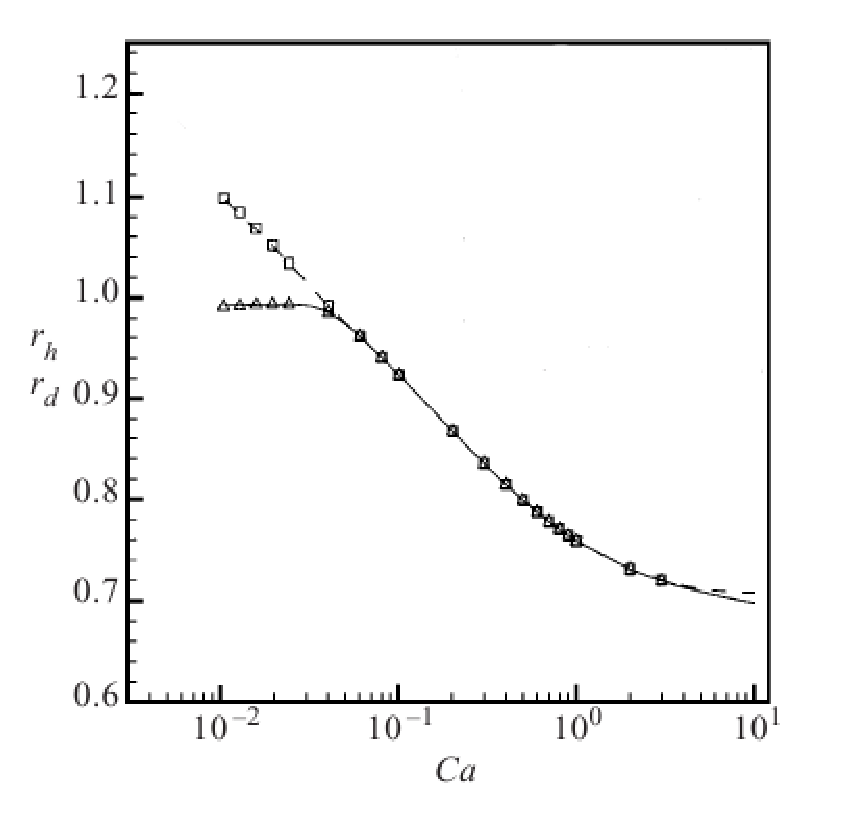
\includegraphics[width=\textwidth]{Figures/capillary_width_heil.eps}
\caption{\citet{heil-threedim} results for the variation of the deposited liquid for the range of
capillary number. One can see the asymmetry between diagonal and axis diameter for the capillary
number $Ca\leq\hat{Ca}=0.04$. Courtesy of \citet{heil-threedim}. \label{fig:heil:three:dim}}
\end{figure}
The transition number between non-axisymmetric case and symmetric is indicated in a number of
works as $\widehat{Ca}=0.04$ \cite{cerro-bubble-train},
$\widehat{Ca}=0.1$
\cite{cerro-space,wang-non-circular}, $\widehat{Ca}=0.033$ \cite{heil-threedim}. If the capillary
number is larger
than
the critical capillary number, i.e. $Ca>\widehat{Ca}$, then the bubble becomes axisymmetric with the
radius of the droplet dependant on the capillary number. One of the example for the bubble radii
dependence on the capillary number is in Fig. \ref{fig:heil:three:dim}.

There are also a number of numerical works for the three-dimensional case. For instance, 
\citet{wong-films,wong-pressure} studied
three-dimensional bubbles in
polygonal capillaries and calculated bubble shapes for different
slug and bubble cross sections and menisci appearance.
\citet{heil-threedim} performed three-dimensional simulations for circular shaped,
square and rectangular shaped capillaries. They indicated the transition
capillary number where the streamlines pattern
changes from having a vortex in front of the bubble and not having it for larger capilllary
numbers, {\color{red} Fig. \ref{fig:streamlines:pattern} }. For the square channel the critical
capillary number is $Ca=0.691$.  Authors also found an empirical correlation which
allows to put
different aspect ratio rectangular channels simulation results on one
curve. It is also indicated that for certain aspect ratio microchannels $\alpha=\frac{a}{b}\geq
2.04$ the interface can not make up the
axisymmetric case for any capillary number. \citet{wang-non-circular} performed numerical
simulations by the VOF technique for the
non-circular
shaped capillaries as square and triangular shaped capillaries. They also investigated the relative
velocity of the bubble for
different capillary numbers. 

As it is mentioned by \citet{gupta-review}, the most common techniques to simulate the Bretherton
phenomena are the Volume of Fluid (VOF) method \cite{wang-non-circular}, the level-set method
\cite{fukugata-levelset} and the finite element methods \cite{kreutzer-taylor,heil-threedim}. It is
also indicated \cite{gupta-review}, that the new techniques which are still in the development stage
are the lattice Boltzmann method and phase field methods \cite{anderson-diffuse,gurtin-binary}.
While the finite element methods solve the Bretherton flow as a free-surface problem with a sharp
interface but without underlying details for gas, the lattice Boltzmann method which is a continuous
interface method arises as a promising alternative for simulation of gas finger propagation. The
continuous interface has more flexebility in simulations involving coalescence and/or droplet
breakup.

In our previous work \cite{kuzmin-binary2d} we already covered the Bretherton flow between plates.
It was shown that the free-energy binary liquid model, which is a phase field method, simulates
with reasonable accuracy the Bretherton/Taylor phenomenon. The goal of this work is to examine the
three-dimensional geometry simulations conducted by the free-energy binary liquid lattice Boltzmann
method. We focus on the feasibility study of the numerical method for the microchannels with
square crosssections. 


The lattice Boltzmann method has emerged as a successful method to simulate
a wide variety of phenomena including hydrodynamics \cite{yu}, thermal flows
\cite{karlin-minimalmodels}, microflows \cite{ansumali-small-knudsen},
ferrofluids \cite{kuzmin-aniso}, and multiphase flows
\cite{swift,Shan-chen:extended}. The method is a particle method which allows to simulate physical
phenomena on the microscopic level. For instance, the introduction of the force or potential on the
microscopic level allows to restore multiphase macroscopic equations \cite{swift,
Shan-chen:extended}.

The binary liquid free-energy LB model due to \citet{swift} we used
simulates two liquids with the assumption of uniform overall
density. While the classical Bretherton problem is stated for gas and liquid, which are of
significantly
different densities and viscosities, the parameters were carefully chosen as to neglect the inertia
effects, see Section \ref{sec:numerical:benchmark}. Moreover, the results of
\citet{giavedoni-numerical} and \citet{heil-bretherton} show
negligible Reynolds number effects on the film thickness for a relatively wide range of Reynolds
numbers. Thus, a major governing factor for microchannel flows is not the density ratio, but
the
viscosity ratio. That is why the uniform density binary liquid model is suitable for this kind of
simulations. The goal of this work is to do a feasibility study of the LBM
binary-liquid model to simulate and correctly predict flow patterns for the Bretherton/Taylor
problem. The work results are in good agreement with other simulations
\cite{heil-threedim,wang-non-circular}. 

One should also acknowledge the works of \citet{pagonabarraga-fingers} on menisci
in thin films for fingering phenomena. \citet{sehgal-microchannel} performed lattice Boltzmann
simulations of two-dimensional channel flows for relatively large capillary numbers, and
found discrepancies with the classical Bretherton theory, which
is limited to the low capillary number regime \cite{giavedoni-numerical}. The Shan-Chen model was
used to simulate the Bretherton problem, which is sometimes referred to contain thermodynamically
inconsistent interface \cite{nourgaliev-breakup}. 

The paper is organized as follows.  First, we explain the simulation benchmark construction
mainly based on our previous work \cite{kuzmin-binary2d}. Then, the binary liquid lattice
Boltzmann model is outlined. The simulation results for the three-dimensional case are presented in
the results section. The results cover the film thickness dependency on the capillary number, the
relative velocity of the bubble and the vortex profiles. The paper
is concluded with a summary of the main findings.
%The critical capillary numbers for changing velocity pattern depending on the eccentricity
%parameter $\alpha$ are presented in Table \ref{table:recirculation:data}.
%\begin{table}
%\begin{tabular}{c|c}
%$\alpha$& $Ca_{T}$\\
%\hline
%1& 0.691\\
%1.1 & 0.688\\
%1.3 & 0.666\\
%1.5 & 0.631\\
%\end{tabular}
%\caption{The results for the recirculation region.\label{table:recirculation:data}}
%\end{table}

\section{Numerical benchmark approach}
\label{sec:numerical:benchmark}
The main discussion here follows and is based on the two-dimensional benchmark approach
\cite{kuzmin-binary2d}. It was indicated that the benchmark layout should have certain
dimensions to conduct simulations. The classical Bretherton benchmark layout is represented in Fig.
\ref{fig:classical:benchmark}. It describes the gas finger propagation through the liquid media.
The film thickness in this case is measured at the inlet. In lattice Boltzmann framework such
formulation has certain challenges \cite{kuzmin-binary2d}. Some of them are attributed to the
dynamic coupling of the inlet and outlet conditions \cite{giavedoni-numerical}. Instead, we
proposed the numerical benchmark indicated in Fig. \ref{fig:lbm:benchmark}. The dimensions of the
channel are chosen as $H_{\mathrm{eff}}\times H_{\mathrm{eff}} \times 15 H_{\mathrm{eff}}$. The
initialized bubble length is taken as $5 H_{\mathrm{eff}}$. \citet{giavedoni-numerical} showed that
the film stabilizes at the distances of $2.6-4.0$ diameters
from the front tip depending on the Reynolds number. \citet{heil-threedim} measure the bubble radii at the distance as $5.5 H_{\mathrm{eff}}$ to be sufficient for $Ca\leq 10$. In this work the conducted simulations capillary number is not larger than unity $Ca\leq 1$.  Thus, the film thickness is chosen to be measured in the
middle of the bubble, which is located at least at a distance of $2.5-3$ channel heights from the 
bubble tip.%at the distances one channel height from the rear tip upto one channel

For simplicity, the periodic boundary conditions are applied. Thus, the bubble train is simulated.
To avoid the mutual influence of bubbles on each other the channel length was chosen as $15
H_{\mathrm{eff}}$. Periodic boundary conditions imply as well that the fluid is accelerated by a
body force in the framework of the LBM but not with the pressure difference. Therefore, we can not
address simulations with upward and downward flows \cite{cerro-bubble-train}. It is assumed that
the gravity effects are negligible and the flow is in the horizontal direction driven by the body
force. 
\begin{figure}[h]
\includegraphics*[bb=153 610 405 717,width=\textwidth]{Figures/benchmark_classical.eps} 
\caption{The classical benchmark layout is presented . The semiinfinite gas bubble
propagates through the liquid media. The inlet pressure is specified $P_{in}$, the outlet is the
free outflow. The bubble propagates with constant velocity $U_{\mathrm{bubble}}$. 
\label{fig:classical:benchmark}}
\end{figure}
\begin{figure}[h]
\includegraphics*[bb=152 470 410 713,width=\textwidth]{Figures/benchmark_lbm.eps}
\caption{The lattice Boltzmann benchmark layout is used in present calculcations. The dimensions of
the domain are chosen as $H_{\mathrm{eff}}\times H_{\mathrm{eff}}\times 15 H_{\mathrm{eff}}$. The
length of the bubble was chosen as $5 H_{\mathrm{eff}}$ for the film thickness to stabilize.
Periodic boundary conditions are applied in the streamwise direction. The flow is driven by body
force. \label{fig:lbm:benchmark}}
\end{figure}

It was indicated \cite{kuzmin-binary2d} that the film thickness for two-dimensional simulations should be at least as twice large
as the interface thickness. The interface thickness in the continuous formulation of the
free-energy binary liquid formulation occupies $3-5$ nodes. Therefore, the film should be
resolved at least as $6-10$ nodes. 

\cite{heil-threedim} specify that the diagonal bubble radius is different from the
axial bubble radius for $Ca\leq \widehat{Ca}\approx 0.05$. The radii coincide for larger values of
$Ca$, but the value of bubble radii is $R_{diag}=R_{axis}=0.99 H_{\mathrm{eff}}$. Therefore, taking the minimal requirement for the film thickness to be
resolved, i.e. $6$ lattice nodes, one can obtain the grid size as $600\times 600 \times 9000 $ to properly resolve the binary liquid microchannels bubbles motion. This size implies highly computational resource to be available for simulations.

One can argue that the non-uniform grid can be used. However, the deposited film thickness is the function of the curvatures of the front bubble tip \cite{bretherton}. Therefore, the grid needs to be refined just at the interface between gas and liquid. It is complicated to achieve for the dynamic systems where a bubble moves in the streamwise direction.

Also, the binary liquid model is used. The model has an uniform density. A part of discussion is addressed in the introduction that to fully address the Bretherton problem one needs to take into the account gravitational, viscous, inertial, and surface tension forces. However,  \citet{shikazono-square} indicated that for square shaped capillaries radii have the
following dependency on the capillary number $Ca$ and the Weber number $We$:
\begin{equation}
\label{radii:experimental}
\begin{aligned}
&R_{diag}=1.171-\frac{2.43 Ca^{2/3}}{1+7.28 Ca^{2/3}-0.255 We^{0.215}}\\
&R_{axis}=
\begin{cases}
1, &R_{diag}>1\\
R_{diag}, &R_{diag}\leq 1.
\end{cases}
\end{aligned}
\end{equation}
Equation (\ref{radii:experimental}) shows that a change in the Reynolds number $0\leq Re \leq 100$ implies the change of the radii from $R_{diag}=R_{axis}=0.96$ to $0.93$ for $Ca=0.1$ and from $R_{diag}=R_{axis}=0.88$ to $0.85$ for $Ca=0.1$. The error of $3$ percent of the channel height is acceptable for current simulations where the Reynolds number is less than {\color{red}$100$}.

Thus, having limitations of the computational memory and performance requirements the focus of the present work is a feasibility study of the binary liquid lattice Boltzmann method for the microchannel simulations with square crossections conducted in the moderate capillary number range $0.1 \leq Ca \leq 1.0$. We base our work on comparison with the already available studies. 

To further reduce the computational overhead only quarter of the channel is simulated, see Appendix
\ref{append:sym}. The next section briefly explains the binary liquid lattice Boltzmann model. Then
the steady-state approach, the dependency of the radii on the moderate capillary number values
$0.1\leq Ca \leq 1.0$, the velocity pattern, the relative bubble velocity and the aspect ratio are
examined, see Section \ref{sec:results}.

\section{Binary liquid lattice Boltzmann model}
The lattice Boltzmann equation (LBE) operates on a rectangular grid representing the
physical domain. It utilizes
probability distribution functions (also known as particle populations)
containing information about
macroscopic variables, such as fluid density and momentum. LBE consists of
two parts: a local collision step, and a propagation step which transports
information from one node to another in certain
directions specified by the discrete velocity set.
The LBE is typically implemented as follows \cite{ginzburg-boundary-main}:
\begin{equation}
\label{standard:implementation}
\begin{aligned}
&f_i^{*}(\bm{x},t)=\omega f_i^{eq}(\bm{x},t)-(1-\omega) f_i(\bm{x},t) +
F_i,&&\text{collision step}\\
&f_i(\bm{x}+\bm{c_i},t+1)=f_i^{*}(\bm{x},t),&&\text{propagation step}, 
\end{aligned}
\end{equation}
where $f_i$ is the probability distribution function in the direction $\bm{c_i}$, $\omega$ is the
relaxation parameter, and $F_i$ is the external force population. The external force population
mimics the force behavior, Eq. \ref{full:navier:stokes}.

The binary fluid LB model is
based on a free-energy functional \cite{swift,landau}, and operates with two
sets of populations: one to track the pressure and the velocity fields, and another to represent the
phase field $\phi$ indicating gas or liquid.
The equilibrium populations \cite{pooley-contact} are defined as:
\begin{equation}
\label{set:equilibrium:binary}
\begin{aligned}
&f_i^{eq}&&=w_i 
\biggl(3
p_0 - k \phi \Delta \phi
+\frac{u_{\alpha}c_{i\alpha}}{c_s^2}+\frac{Q_{i\alpha\beta}u_{\alpha } u_ {
\beta}}{2 c_s^4}\biggr)\\
&&&+k w_i^{\alpha\beta} \partial_{\alpha} \phi\partial_{\beta} \phi, 1\leq i \leq Q-1\\
&f_0^{eq}&&=\rho-\sum_{i\neq0}{f_i^{eq}}\\
&g_i^{eq}&&=w_i\left(\Gamma \mu + \frac{\phi c_{i\alpha} u_{i\alpha}}{c_s^2}+\phi
\frac{Q_{i\alpha\beta}u_{\alpha}u_{\beta}}{2 c_s^4}\right), \leq i \leq Q-1\\
&g_0^{eq}&&=\phi-\sum_{i\neq0}{g_i^{eq}}\quad,
\end{aligned}
\end{equation}
where $\Gamma$ is the mobility parameter; the chemical potential
$\mu=-A\phi+A\phi^3-k\Delta\phi$; $k$ is the parameter related to the surface
tension; $A$ is the parameter of the free-energy model; $Q$ is the number of the directions ($9$ and
$19$ for the $D2Q9$ and $D3Q19$ models, correspondingly); the tensor
$Q_{i\alpha\beta}=c_{i\alpha} c_{i\beta} - c_s^2 \delta_{\alpha\beta}$ with
the sound speed parameter $c_s^2=1/3$. The bulk pressure
is expressed as $p_0=c_s^2 \rho +A (-0.5 \phi^2+0.75 \phi^4)$. The particular weights and velocity
sets for the $D2Q9$ and $D3Q15$ models are indicated in Appendix A. 

The set of equations (\ref{set:equilibrium:binary}) restores the macroscopic
fluid equations as:
\begin{equation}
\label{full:navier:stokes}
\begin{aligned}
&\partial_t \rho+ \partial_{\alpha} \rho u_{\alpha}=0\\
&\rho\left(\partial_t+u_{\beta}\partial_{\beta}\right) u_{\alpha}=
-\partial_{\beta}P_{\alpha \beta} +
\nu\partial_{\beta}\left(\rho\partial_{\alpha}u_{\beta}+\rho\partial_{\beta} u_{\alpha}\right)\\
&\partial_t \phi + \partial_{\alpha} \phi u_{\alpha}=M \partial^2_{\beta\beta} \mu,
\end{aligned}
\label{binary:fluid:system}
\end{equation}
where $\nu=c_s^2 (\tau-1/2)$ is the dynamic viscosity,
$M=\Gamma(\tau_{\phi}-1/2)$ is the mobility parameter, and $\tau=\frac{1}{\omega}$ and $\tau_{\phi}$
are the relaxation parameters of density and phase fields. 

The system allows the separation of the liquid
phase with $\phi=1$ and a so-called gas phase with $\phi=-1$. The
relaxation time is taken as linearly dependent on the relaxation
times $\tau_{\mathrm{gas}}$ and $\tau_{\mathrm{liq}}$:
$\tau=\tau_{\mathrm{gas}}+\frac{\phi+1}{2}(\tau_{\mathrm{liq}}-\tau_{\mathrm{gas}})$. This allows
to change viscosity from the gas viscosity
$\nu_{\mathrm{gas}}=\frac{1}{3}\Bigl(\tau_{\mathrm{gas}}-\frac{1}{2}\Bigr)$ to the liquid viscosity
$\nu_{\mathrm{liq}}=\frac{1}{3}\Bigl(\tau_{\mathrm{liq}}-\frac{1}{2}\Bigr)$ while phase changes
accordingly.The surface tension in the framework of the binary liquid model is $\sqrt{\frac{8 k
A}{9}}$.

Velocity set is defined as:
\begin{equation} 
\begin{aligned}
&c_{ix}=\{0,1,-1,0, 0,0, 0,1,-1, 1,-1,0, 0, 0, 0,1,-1, 1,-1\}\\
&c_{iy}=\{0,0, 0,1,-1,0, 0,1, 1,-1,-1,1,-1, 1,-1,0, 0, 0, 0\}\\
&c_{iz}=\{0,0, 0,0, 0,1,-1,0, 0, 0, 0,1, 1,-1,-1,1, 1,-1,-1\}.
\end{aligned}
\end{equation}
The weights are $w_0=0$, $w_{1-6}=\frac{1}{6}$ and $w_{7-18}=\frac{1}{12}$. The weights
related to the inclusion of the surface tension are:
\begin{equation}
\begin{aligned}
&w^{xx}_{1-2}=w^{yy}_{3-4}=w^{zz}_{5-6}=\frac{5}{12}\\
&w^{xx}_{3-6}=w^{yy}_{1-2,5-6}=w^{zz}_{1-4}=-\frac{1}{3}\\
&w^{xx}_{7-10,15-18}=w^{yy}_{7-14}=w^{zz}_{11-18}=-\frac{1}{24}\\
&w^{xx}_{11-15,}=w^{yy}_{15-18}=w^{zz}_{7-10}=\frac{1}{12}\\
&w^{xy}_{7,10}=-w^{xy}_{8,9}=w^{yz}_{11,14}=-w^{yz}_{12,13}=w^{zx}_{15,18}=-w^{zx}_{16,17}=\frac{1}{
4}.
\end{aligned}
\end{equation}


\section{Results}
\label{sec:results}
This section describes numerical simulations. First, we examine when the steady-state approach is
achieved. Then, the critical capillary number is identified when the transition from the
non-symmetrical to axisymmetrical bubble shape occurs. The dependency of the radii on the capillary
number is presented for the range of moderate capillary numbers $0.1 \leq Ca 1.0$. Results are
concluded with studies of the velocity pattern,{\color{red} the aspect ratio, and the influence of
inertia}.


\subsection{Steady-state approach}
We performed different simulations to understand a number of steps required for the problem to come
on the steady-state. The grid to be simulated is $52\mathrm{x}52\mathrm{x}750$ which simulates the
quarter of the channel with the initial
width as $6.5$ lattice Boltzmann units together with the body force as
$\frac{\mathrm{d}P}{\mathrm{d}x}=1.6
\mathrm{x}10^{-6}$. The simulation was performed for $140000$, $160000$, $180000$, $200000$,
$220000$ and
$240000$ iterations. The results are summarised in Table \ref{table:steady:state}. Whole the
capillary number varies only in the 4th digit, radiuses are one percent accurate. 
\begin{table}
\begin{tabularx}{\textwidth}{|X|X|X|X|}
\hline
$N_{iter}$&$Ca$&$R_{axis}$&$R_{diag}$\\
\hline
$140000$&$0.1879$&$0.8657$&$0.8708$\\
$160000$&$0.1878$&$0.8650$&$0.8702$\\
$180000$&$0.1882$&$0.8647$&$0.8700$\\
$200000$&$0.1893$&$0.8645$&$0.8698$\\
$220000$&$0.1925$&$0.8644$&$0.8697$\\
$240000$&$0.1961$&$0.8645$&$0.8697$\\
\hline
\end{tabularx}
\caption{Results for the steady-state case. One
can see that $200000$ steps are enough to structure
the bubble and approach the steady state. The small noise in the capillary number is connected to
the identification of the interface. One needs to address the interpolation and the spurious
currents existing in the system. All other parameters are relaxed to the
steady-state.\label{table:steady:state}}
\end{table}

To further examine the steady-state the velocity in the streamwise direction is plotted. The values
of the velocity are taken on the contour where phase values are taken as $\phi=0$. This corresponds
 to the bubble interface. One can see the contour plot and the corressponing streamwise velocity
component in Fig. \ref{fig:velocity:contour}. The crossection is a plane $x=0$, where $x$ points
towards the reader, $z$ is the streamwise direction. As far as fluxes inside the bubble has
clockwise and counterclockwise directions, see Section \ref{sec:velocity}, one needs to thoroughly
examine only the points corresponding to the front and the rear bubble tips. If one finds it equal
to each other, then it's exactly the velocity with which the bubble propagates in the microchannel. 
\begin{figure}[h!]
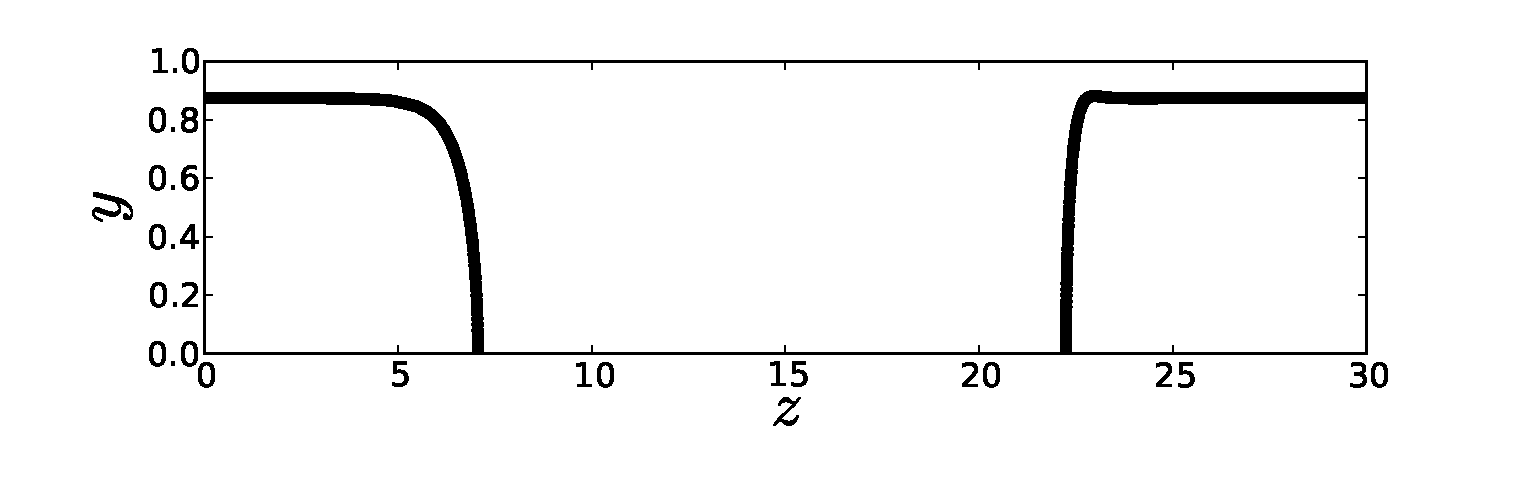
\includegraphics[width=\textwidth]{Figures/velocity_interface_contour.eps}\\
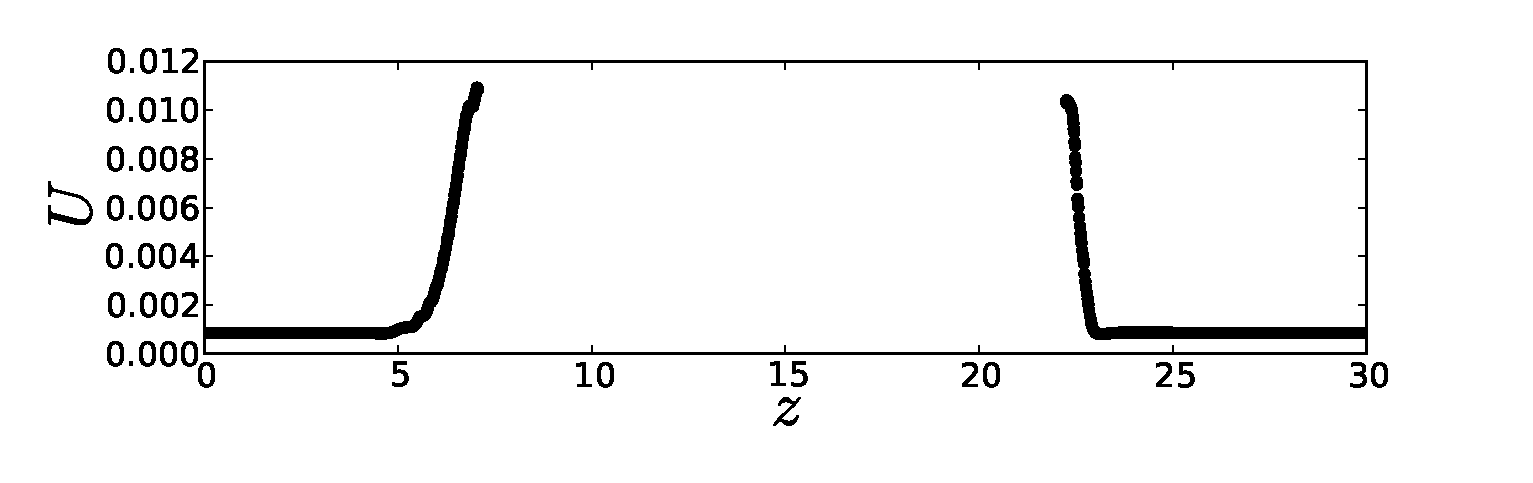
\includegraphics[width=\textwidth]{Figures/velocity_interface_values.eps}\\
\caption{The bubble shape and the corresponding streamwise velocities taken on the bubble
interface after $240000$ iterations. Directions $y$ and $z$ are scaled to the half of the channel
$H_{\mathrm{eff}}/2$. One can see that the bubble front and rear tips are propagating with the
same velocities, which is actually the bubble velocity. For more details on velocity patterns
see Section \ref{sec:velocity}. \label{fig:velocity:contour}}
\end{figure}


\subsection{Radii transition}
Due to performance issues we can only access the
transition region, i.e. $Ca\geq 0.05$. In this region the proper resolution of the film thickness
is guaranteed. To identify the critical capillary number $\widehat{Ca}$ a number of simulations
were conducted. Surprisingly the transition occurs in the region computationally accessible for
current simulations. In comparison with the results of the \citet{heil-threedim}
($\widehat{Ca}=0.04$) our
results are more close to the VOF continuous interface method simulation by
\citet{wang-non-circular} ($\widehat{Ca}=0.1$) and experimental dependency of
\citet{shikazono-square}, see Table
\ref{table:transition:results}. The transition happens for $Ca\approx 0.09$.  One can see
two examples of non-symmetric and axisymmetric bubble shapes for $Ca=0.053$ and $Ca=1.13$, see Fig.
\ref{fig:crosssections:sym}.  
\begin{table}
\begin{tabularx}{\textwidth}{|X|X|X|X|X|X|}
\hline
$Ca$&$R_{axis}$&$R_{diag}$&$Re$&$R_{axis,Wang}$&$R_{diag,Wang}$\\
\hline
$0.053$&$0.95$&$1.01$&$0.907$&$0.99$&$0.99$\\
$0.078$&$0.93$&$0.95$&$1.062$&$0.96$&$0.96$\\
$0.132$&$0.89$&$0.89$&$1.80$&$0.93$&$0.93$\\
\hline
\end{tabularx}
\caption{Simulation results in terms of $R_{axis}$ and $R_{diag}$ for the transition region between
non-symmetric and axisymmetric cases. $R_{axis,Wang}$ and $R_{diag,Wang}$ are experimental
correlations by \citet{wang-non-circular}. \label{table:transition:results}}
\end{table}
\begin{figure}[ht]
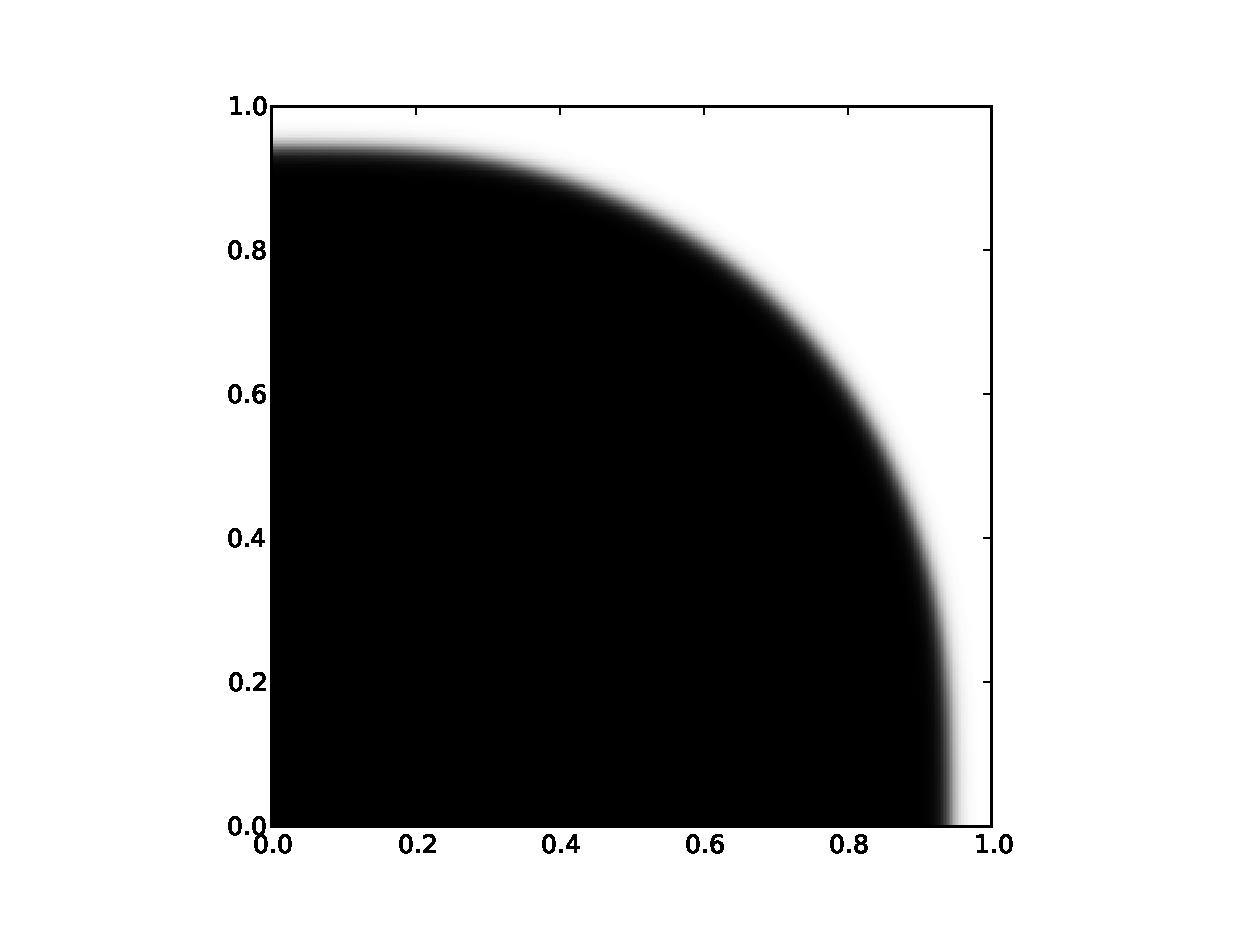
\includegraphics[width=0.5\textwidth]{Figures/phase_crossection_ca5.eps}
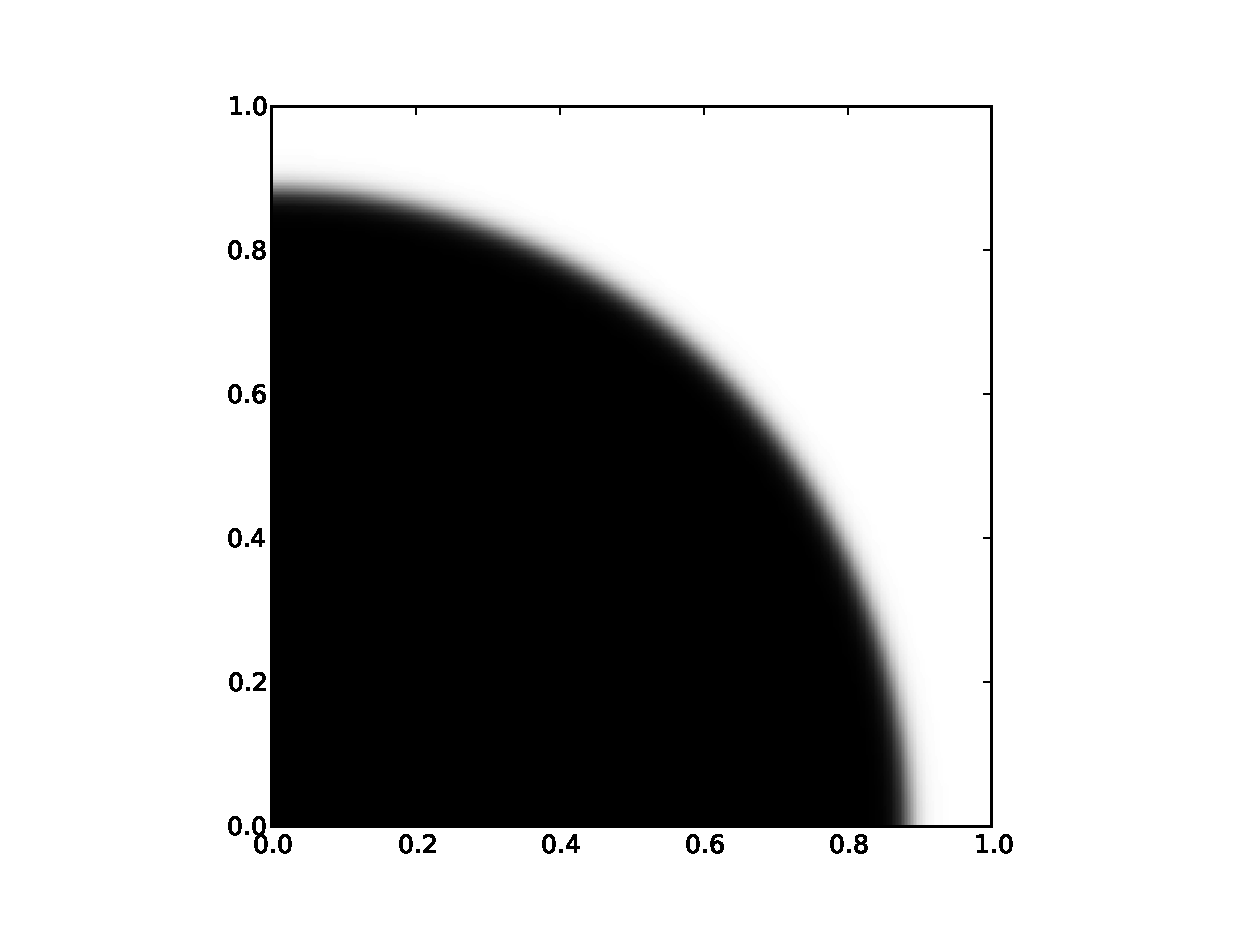
\includegraphics[width=0.5\textwidth]{Figures/phase_crossection_ca13.eps}\\
\caption{Crosssections of the phase field in the middle of the bubble for $Ca=0.053$
(left) and $Ca=1.13$ (right). Crosssections are rescaled on the half channel height. Other
parameters are indicated in Table \ref{table:transition:results}. One can see that the left picture
is asymmetric in comparison
with the right one. The transition happens for $Ca\approx 0.09$.\label{fig:crosssections:sym}}
\end{figure}


\section{Velocity pattern}
\label{sec:velocity}
The velocity pattern is known to change its behavior depending on the capillary number. For
relatively low capillary number $Ca<0.6$ there exists a vortex in front of the bubble in the moving
frame moving with the bubble \cite{heil-threedim}. For larger ones it is indicated that there is no
vortex in front of the bubble. The transition capillary number is indicated by
\citet{heil-threedim} and it equals for the rectangular channel $Ca=0.691$. However, the
distribution of vorticity strongly depends on Reynolds number \cite{heil-bretherton}, as well the
pressure distribution. In the case of the bubble train it is indicated by \citet{kreutzer-taylor}
that the pressure is largely influenced by bubble frequency and slug distance. The present
simulations are conducted for bubble trains and certain differences in terms of changing streamline
patterns are expected. We examined velocity patterns to identify the moment of the streamlines
pattern change. We chose two
representative capillary numbers as $Ca=0.47$ and $Ca=0.63$. 
One can
see a clear transition between associated patterns. The transition capillary number
\cite{heil-threedim} is slightly higher than the simulation results. In present simulations the
transition occurs at $Ca=0.5-0.6$.
\begin{figure}[h]
\includegraphics[angle=90,width=\textwidth]{Figures/stream_ca47.eps}\\
\includegraphics[angle=90,width=\textwidth]{Figures/stream_ca63.eps}\\
\caption{Velocity vector maps for $Ca=0.47$ and $Ca=0.63$. One can see that there are no vortexes
created
before the bubble for $Ca=0.63$. The transition happens between $Ca=0.47$ and $Ca=0.63$, which
is a different value from $Ca=0.69$ \cite{heil-threedim}. \label{fig:streamlines:pattern}}
\end{figure}


\section{Variation bubble length}
The work of \citet{wang-non-circular} shows the variation of the bubble
thickness through the length of
bubble. The bubble shape in terms of axial and diagonal radii is reconstructed for a number of
capillary numbers, Fig. \ref{fig:bubble:variation:capillaries}. One can see that for smaller
capillary numbers the diagonal radius exhibits a small jump near the rear bubble tip. It coincides
with results of \citet{wang-non-circular}. However, present simulations show smoother behavior of
the jump.  
\begin{figure}[h]
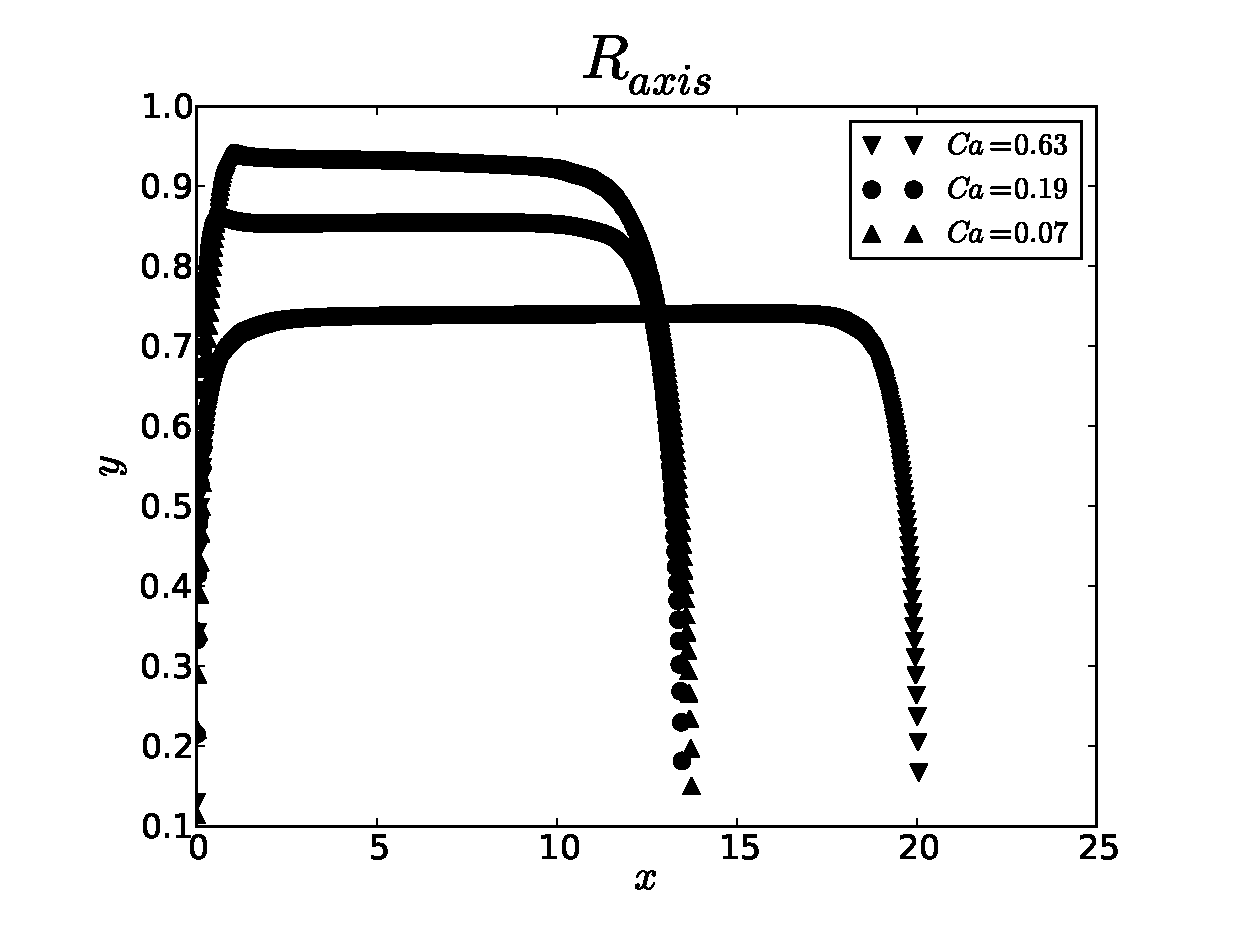
\includegraphics[width=\textwidth]{Figures/bubble_rad_axis.eps}\\
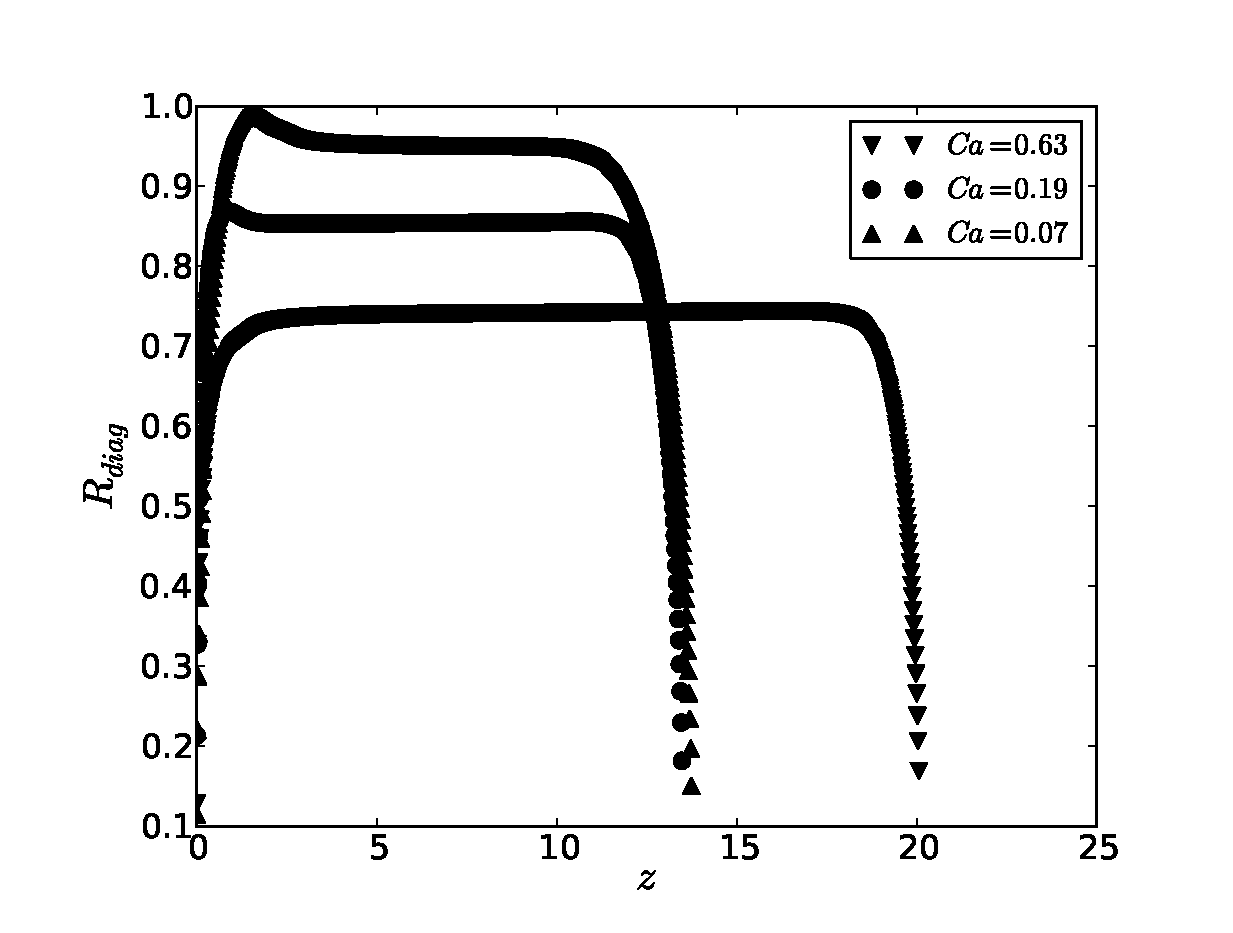
\includegraphics[width=\textwidth]{Figures/bubble_rad_diag.eps}\\
\caption{Radii variations along the bubble for different capillary numbers in the plane $x=0$.
One can see that the diagonal radius shows the jump near the bubble rear tip. It coincides with the
VOF simulations of \citet{wang-non-circular}. \label{fig:bubble:variation:capillaries}}
\end{figure}

Another interesting phenomenon for the bubble shape was indicated by \citet{heil-threedim}. In
their simulations the non-symmetric shape was observed even for larger capillary number $Ca>4$ near
the bubble front tip. We performed the same simulations. 


\begin{figure}
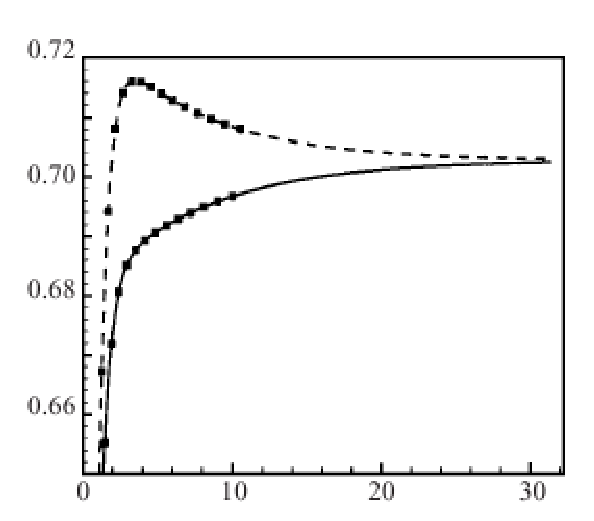
\includegraphics[width=0.97\textwidth]{Figures/variationoverlength.eps}
\caption{The variation of the bubble length for capillary number $Ca=10$. The x-axis scaled to
half-width of the microchannel height.  \label{fig:thickness:variation:ca:ten}}
\end{figure}

Concerning results indicated in Fig.
\ref{fig:thickness:variation:ca:ten} simulations are unstable that means one needs to work with
small surface tension ({\color{red} See results of Pagonabarraga}). One can see that the difference
between diagonal radius and
usual radius is of order of $4\%$. That means it's 2 percent of the channel height. If the
simulation is conducted by the grid $100\mathrm{x}100$ in the cross section that means that we will
see the difference in two grid nodes. Therefore the grid is $102\mathrm{x}102\mathrm{1500}$. It is
known from simulations that for the grid $102\mathrm{x}102\mathrm{x}1500$ the largest force gradient
is $2\mathrm{x}10^{-5}$ with free energy binary liquid parameters $A=0.04$,$k=0.04$ and $Ca\approx
1.0$. Therefore, we want to keep the same body force but to obtain larger capillary number. That
can be done through the scaling indicated in Appendix \ref{append:scaling}:
\begin{equation}
\frac{\mathrm{d}P}{\mathrm{d}x}\propto \gamma Ca .
\end{equation}
Therefore the same body force can stand for capillary number ten times larger if the surface
tension is ten times smaller:
\begin{equation}
\gamma=\sqrt{\frac{8 k A}{9}}.
\end{equation}
The following can be satisfied if $A=0.004$ and $k=0.004$. Decreasing surface tension requires
increasing the mobility of the interface to be able to adjust to the interface
\cite{pagonabarraga-parameters}. We therefore performed the numerical simulation with those
parameters and $\Gamma=20$ for the interface to be stable. 
{\color{red} However, many authors state that increasing mobility kills
the
proper results of simulations}.
{\color{red} Need to wait results from bugaboo.westgrid.ca under LargeCap simulation}

\section{Capillary number}

While changing the applied force in a manner indicated in Appendix
\ref{append:scaling} the velocity of the bubble was increased to obtain larger capillary numbers,
see Fig. \ref{fig:underresolved:capillaries}. One can see that the deviation between the diagonal
and axial radiuses are quite significant and they coincide only when the interface is resolved
($Ca\approx 1.0$). In calculations with better grids, i.e. quarter channels simulations on CPU, the
axial radius coincides with the diagonal in the $0.5\%$ range. Moreover, the capillary number curve
resembles already published date of \citet{heil-threedim} in a better way, see Fig.
\ref{fig:capillary:comparison}. 




We performed a number of simulations with quarter CPU code and GPU train simulations and compared
them with data obtained by \cite{heil-threedim}. After performing the simulations we determine the
$R_{axis}$, $R_{diag}$ versus calculated
capillary number
\begin{equation}
Ca=\frac{\mu_{liq} U_{bubble}}{\gamma}.
\end{equation}
To perform simulations we
started with the following parameters as
$k=0.04$,$A=0.04$,$\Gamma=1.0$. We performed different grids calculations with GPU and CPU codes.
The GPU code (see section \ref{section:bubble:train} about bubble train simulations) simulates a
quarter of the bubble and operates on the grid $100\mathrm{x}100\mathrm{x}1500$. The CPU refined
grid operates on whole $160\mathrm{x}160\mathrm{x}1500$. In this case we see short bubbles as the
length to height ratio is $\frac{500}{160}=3.125$. GPU  For GPU grids due to memory constrains we
chose the grid as $N_x\mathrm{x}N_y\mathrm{x}N_z=52\mathrm{x}52\mathrm{x}750$. One can see the
comparison presented in Fig. \ref{fig:capillary:comparison}.
\begin{figure}
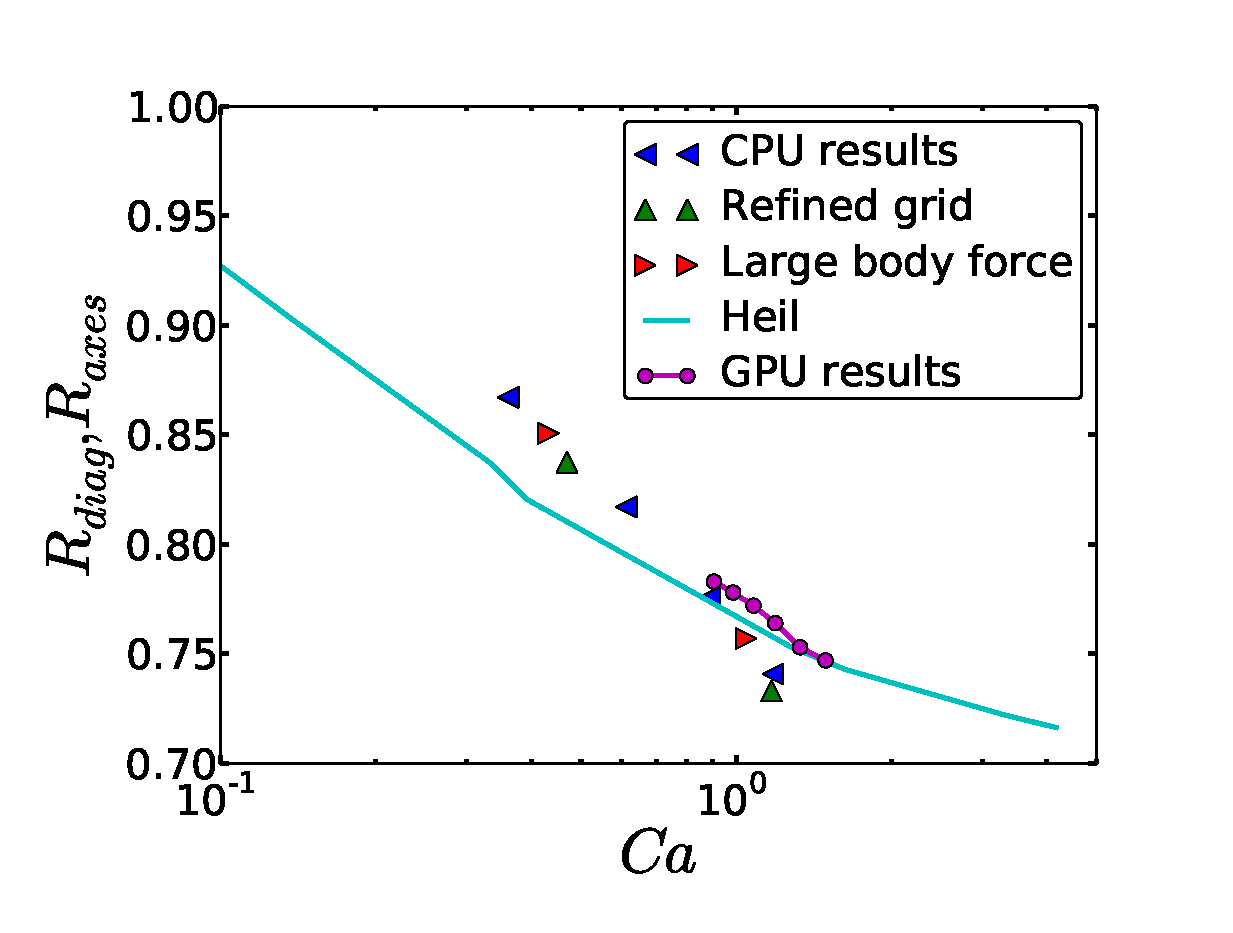
\includegraphics[width=0.97\textwidth]{Figures/capillaries_comparison.eps}
\caption{The comparison between different runs of codes for the axial and the diagonal radiuses
versus capillary numbers. \label{fig:capillary:comparison}}. One can see that the code mimics
behavior of the earlier published results.
\end{figure}


\section{Train simulation}
\label{section:bubble:train}
As far as the requirements for the grid are ``heavy'' we performed a bunch of simulations to
examine how the distance between bubbles influences on the thickness. For this purpose the
simulation was conducted on the grid 82x82x750. We examined different initialized distances between
bubbles. The initial lengths of bubbles were chosen as $300$, $350$, $400$, $450$, $500$, $550$
lattice units. Therefore, the corresponding initial distances between bubbles are
$450$,$400$,$350$,$300$,$250$ lattice units. On the steady state regime the distances become $386$,
$317$, $248$,$176$,$99$,$23$ lattice units. The corresponding capillary numbers calculated based on
the center bubble velocity are as follows $0.905$, $0.986$,$1.08$,$1.19$, $1.33$, $1.49$. The
calculated radiuses (diagonal radius equal to the axes radius) are as follows
$0.783$,$0.778$,$0.772$,$0.764$,$0.753$,$0.747$. Thus, one can see the great impact of the bubbles
on each other velocity for the given body force. However, in terms of the film thicknesses those
numbers look adequate. One can see the film thicknesses dependency on the capillary number for
simulations obtained by \citet{heil-threedim} and bubble train simulations data in Fig.
\ref{fig:capillaries:train} and in Fig. \ref{fig:capillary:comparison}. One can see that the
results are consistent and in a good agreement.
Therefore, though the bubble train mutual motion influences on the film thickness by increasing the
associated capillary number,  however, the film thickness is in accordance with the capillary
number correlation. Thus, the decrease of the numerical domain is quantified and can be used to
obtain the data. However, one should be cautious about the initialization, because the Poiseuille
flow initialization is deviated even further due to mutual motion of bubbles.
\begin{figure}
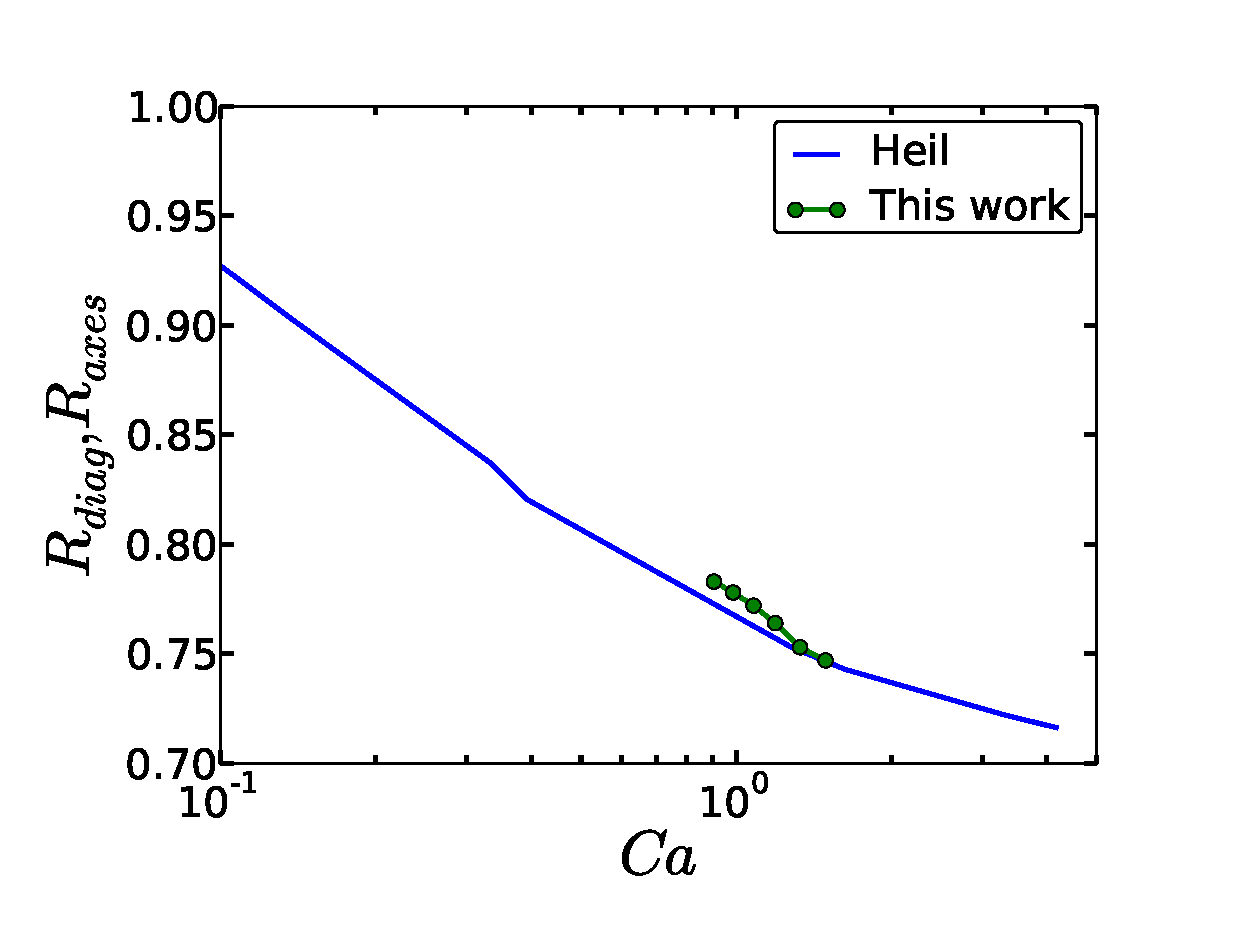
\includegraphics[width=0.97\textwidth]{Figures/capillaries_comparison_train.eps}
\caption{The comparison for the film thickness between \citet{heil-threedim} data and bubble train
simulations. Though, one can see that the decrease of the distance between bubbles causes the
increase in the associated capillary number, however, the correlation dependance between film
thickness and capillary number stays the same. This can help for simulations to reduce the
numerical domain. \label{fig:capillaries:train}}
\end{figure}

\section{Conclusion}
The present work conducts the binary-liquid simulations with the lattice Boltzman method. The
method is a continuous interface method. Along with similarity of results with already published
results of \citet{heil-threedim} and \citet{wang-non-circular}, the differencies were found,
especially in the velocity pattern. Results evedince that the lattice Boltzmann binary liquids
simulations can be used for simulation of gas bubbles in the microchannel. 

\appendix
\section{Symmetric boundary conditions}
\label{append:sym}
For the memory save we performed the simulation of the quarter of the channel while using the
antisymmetric boundary conditions. In the macroscopic variables the mirror boundary conditions
require to have the same scalar fields, but for velocity only tangential velocities are the same
but perpendicular have the opposite directions. This implies the following in terms of the
macroscopic variables:
\begin{equation}
\rho_B = \rho_F, \quad \phi_B = \phi_F \quad U_{B\tau}=U_{F\tau}, U_{B n}=U_{F n}, 
\end{equation}
 where $B$ and $F$ stand for the boundary and the nearest fluid node, respectively. 

In terms of the lattice Boltzmann populations this conditions require the same set of the
populations for the boundary node as for the fluid node. However, the set is mirrored against the
plane of the boundary. This case allows to conserve scalar fields, to have the same tangential
velocities and to have opposite normal velocities. The grid was chosen as 52x52x1500, which is the
effective calculated domain as 100x100x1500 grid nodes. 

\section{Scaling procedure}
\label{append:scaling}
For scaling purposes one need to obtain setup a body force as $\frac{\mathrm{d}P}{\mathrm{d}x}$. If
one obtained a certain velocity of the bubble with the associated gradient then another gradient
can be obtained through the porpotionality condition as:
\begin{equation}
\frac{\mathrm{d}P}{\mathrm{d}x}=\frac{8}{N_y^2} \gamma Ca,
\end{equation}
or in other words th functionality can be extended as:
\begin{equation}
\dfrac{\dfrac{\mathrm{d}P_1}{\mathrm{d}x}}{\dfrac{\mathrm{d}P_2}{\mathrm{d}x}}=\frac{Ca_1}{Ca_2}
\frac{N_{
y2}^2 }{N_{y1}^2}
\end{equation}


\bibliographystyle{unsrtnat}
\bibliography{paper}
\end{document}


